\documentclass[11pt]{article}
\usepackage{cse103}
\def\title{HW 2}

% use the tikz package to draw automata
\usepackage{tikz}
\usetikzlibrary{arrows,positioning,automata}

\begin{document}
\maketitle

\section*{Due October 13 at 11:59pm}

\textbf{(5 questions, 235 points total)}

\begin{qunlist}

  \q{50}{Proving a DFA has a particular language}\\
  Suppose we have a robot which moves around in a 1D world, moving either left or right at each time step.
  We can represent its trajectory as a string over the alphabet $\Sigma = \{ \leftarrow, \rightarrow \}$: for example the string $\leftarrow \leftarrow \rightarrow$ would mean that the robot moves left twice, then right once.
  Suppose that if the robot moves more than $k$ steps left or right of its starting position, it will fall off a cliff and get stuck.
  Let $L_k$ be the language of all trajectories where the robot does \emph{not} fall; then for example $L_1$ would contain $\rightarrow \leftarrow$ but not $\rightarrow \leftarrow \rightarrow \rightarrow \leftarrow$, since in the latter trajectory the robot falls off the cliff after the 4th movement.

  We can build a DFA recognizing $L_k$, but we can't draw it as a graph since $k$ is arbitrary and we'll need a different DFA $M_k$ for each $k \ge 0$.
  So we'll define $M_k = (Q_k, \Sigma, \delta_k, q_0, F_k)$ mathematically, as follows:

  \begin{itemize}
    \item $Q_k = \{ q \in \Z \st |q| \le k+1 \} = \{ -(k+1), -k, \dots, -1, 0, 1, \dots, k, k+1 \}$
    \item $\Sigma = \{ \leftarrow, \rightarrow \}$
    \item $\delta_k(q, s) =
            \begin{cases}
              q + 1 & |q| \le k \text{ and } s = \rightarrow \\
              q - 1 & |q| \le k \text{ and } s = \leftarrow  \\
              q     & |q| > k
            \end{cases}$
    \item $q_0 = 0$
    \item $F_k = \{ q \in \Z \st |q| \le k \} = \{ -k, \dots, -1, 0, 1, \dots, k \}$
  \end{itemize}

  Intuitively, this DFA works by using states to keep track of where the robot currently is, updating the state at each time step and getting stuck in a non-accepting state if the robot ever moves too far from the start.
  Notice how we've used integers as states so that we can add or subtract 1 to them to represent the robot moving from one position to the next: you can use any objects as states in a DFA.

  Lets formally verify this intuition, and use it to prove the correctness of our DFA.

  \begin{qparts}
    \item (\emph{40 pts.})
    Prove that $\widehat{\delta_k}(q_0, x)$ (the state reached when running $M_k$ on input $x$) is the position of the robot after following the trajectory $x$, where we consider positions $k+1$ and $-(k+1)$ to indicate having fallen off the right and left cliffs respectively.\\
    (\emph{Hint:} Use induction on the length of $x$.)
    \begin{solution}
      Proof:\newline
      Base case if $x=\epsilon$:
      \begin{equation}
        \widehat{\delta_k}(q_0, \epsilon) = q_0
      \end{equation}
      If there are no moves then the robot's position is the same as the starting position. Which means that the extended transition function being the position of the robot after sequence of moves x holds. We now proceed with the assumption that $\widehat{\delta_k}(q_0,x)$ is the position after sequence of moves x. Then:\newline\newline
      Inductive step:
      \begin{gather}
        \widehat{\delta_k}(q_0,xm) \mbox{ for any $x \in \Sigma^*$ and $m \in \Sigma$}\\
        = \delta_k(\widehat{\delta_k}(q_0,x),m)\\
        \nonumber\mbox{if we assume x to be a string of moves from $\Sigma^*$ then x can be $\epsilon$}\\
        = \delta_k(\widehat{\delta_k}(q_0,\epsilon),m)\\
        = \delta_k(q_0,m) \Rightarrow \mbox{ the position after taking move m from $q_0$}
      \end{gather}
      Therefore the position after the sequence of moves xm can be represented by $\widehat{\delta_k}(q_0,xm)$. Accordingly the position after the sequence of moves x can be represented by $\widehat{\delta_k}(q_0,x)$
    \end{solution}

    \item (\emph{10 pts.})
    Using the result of part (a), prove that this DFA actually works, that is, that $L(M_k) = L_k$.\\
    (\emph{Hint:} Use the lemma stated in class that $M_k$ accepts $x$ if and only if $\widehat{\delta_k}(q_0, x) \in F_k$.)
    \begin{solution}
      Using the lemma from class ($L(M_k) = \{x \in \Sigma^* | \widehat{\delta_k}(q_0,x) \in F_k)\}$), and the fact that $\widehat{\delta_k}(q_0,x)$ results in the position after sequence x we can say that the lemma holds since:
      \begin{gather}
        x = \epsilon\\
        \widehat{\delta_k}(q_0,\epsilon) = q_0 \in F_k
      \end{gather}
      If $x = \epsilon$ then the position will be $q_0$ which falls in the set of final states. Therefore $L(M_k) = L_k$ since the resulting state is in the language $L_k$.
    \end{solution}
  \end{qparts}

  \newpage

  \q{35}{Defining a DFA symbolically}\\
  For a given integer $k \ge 1$, let the language $L_k$ consist of the strings over the binary alphabet $\Sigma = \{0,1\}$ whose $k$th symbol from the end is 1 (so for example $0100 \in L_3$).
  We saw an NFA for $L_3$ in class; we can also build a DFA for $L_k$ (directly, without using the NFA-to-DFA conversion we'll cover later).
  For example, here is a DFA that recognizes $L_2$:

  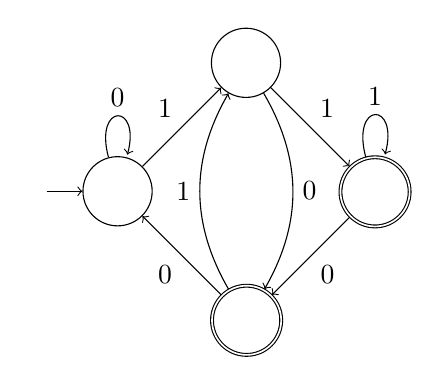
\begin{tikzpicture}
    \node[state, initial, initial text=] (s1) {};
    \node[state, above right= of s1] (s3) {};
    \node[state, accepting, below right= of s1] (s4) {};
    \node[state, accepting, below right= of s3] (s2) {};

    \path[->]
    (s1) edge node[above left] {$1$} (s3)
    (s1) edge[loop above] node[above] {$0$} (s1)
    (s3) edge[bend left] node[right] {$0$} (s4)
    (s3) edge node[above right] {$1$} (s2)
    (s4) edge[bend left] node[left] {$1$} (s3)
    (s4) edge node[below left] {$0$} (s1)
    (s2) edge node[below right] {$0$} (s4)
    (s2) edge[loop above] node[above] {$1$} (s2);
  \end{tikzpicture}

  \begin{qparts}
    \item \emph{(30 pts.)}
    Define a DFA $M_k$ recognizing $L_k$.
    Since $k$ is arbitrary, you can't draw a graph; define the states $Q_k$, transition function $\delta_k$, etc. mathematically, as we did in question (1).
    (You do not have to prove that your DFA recognizes $L_k$, but if you'd like more practice with induction, give it a try!)

    (\emph{Hint:} The states in the set $Q$ don't have to be numbers; any distinct objects are fine. You could have states labeled by English words, for example, and then it would be well-defined to say something like ``all states whose first letter is Z''. So if it's convenient, feel free to have the ``names'' of the states store some useful information rather than just being numbers or letters.)
    % https://inst.eecs.berkeley.edu/~cs172/sp09/s1.pdf
    \begin{solution}
      \begin{gather}
        Q = \{s_q \mbox{ for some } q \in \Sigma^k\}\\
        \Sigma = \{0,1\}\\
        \delta_k(s_q,x) = \begin{cases}
          s_{q0} & \mbox{if }q\in\{0,1\}^{k-1} \mbox{ and } x = 0 \\
          s_{q1} & \mbox{if }q\in\{0,1\}^{k-1} \mbox{ and } x = 1 \\
        \end{cases}\\
        q_0 = s_{1^k}\\
        F = \{s_z \mbox{ for some z that starts with 0}\}
      \end{gather}
    \end{solution}
    \item \emph{(5 pts.)}
    How many states does your automaton have?
    \begin{solution}
      The automaton has $2^k$ states. with $\frac{2^k}2$ accepting states.
    \end{solution}
  \end{qparts}

  \newpage

  \q{35}{Does a DFA accept everything?}
  \begin{qparts}
    \item \emph{(20 pts.)}
    Describe an efficient algorithm to decide whether a DFA $D$ accepts all strings, i.e.~whether $L(D) = \Sigma^*$.
    You may use standard graph algorithms as subroutines.
    % https://cs.stackexchange.com/questions/73993/how-to-determine-if-an-automata-dfa-accepts-an-infinite-or-finite-language
    \begin{solution}
      The algorithm to check if a DFA accepts all strings is to check if the DFA contains loops, howver a DFA containing loops only has a posibility of accepting all strings so if we check to see if the DFA has no loops then we know that the DFA does not accept all strings.
    \end{solution}

    \item \emph{(5 pts.)}
    What is the asymptotic runtime of your algorithm, assuming $D$ has $n$ states and $|\Sigma| = m$?
    \begin{solution}
      The runtime of the solution is $O(n)$ since we have to check every state in the DFA to see if it has a connection to an already checked state.
      Similar to Djikstra's algorithm we have to propogate through the entire graph. But we only check for loops which follows Floydd's Tortise and Hare algorithm for finding loops/cycles in a linked list.

    \end{solution}

    \item \emph{(10 pts.)}
    Would your algorithm also work for an NFA?
    If so, explain why.
    If not, give an example of an NFA where your algorithm returns the wrong answer.
    \begin{solution}
      An NFA will have epsilon transitions and therefore have a loop and along with that if we take into account that there are more possibilites for loops with the fact that NFA's can have multiple paths from start to accepting state given an input the algorithm to check for no loops should fail.
      This does mean that the algorithm is not perfect for NFAs. An example would be an NFA with epsilon transitions to detect if a string contains the substring "ab" or "aba" as the graph can look like the following with loops but not accept all strings:
    \end{solution}
    \begin{align}
      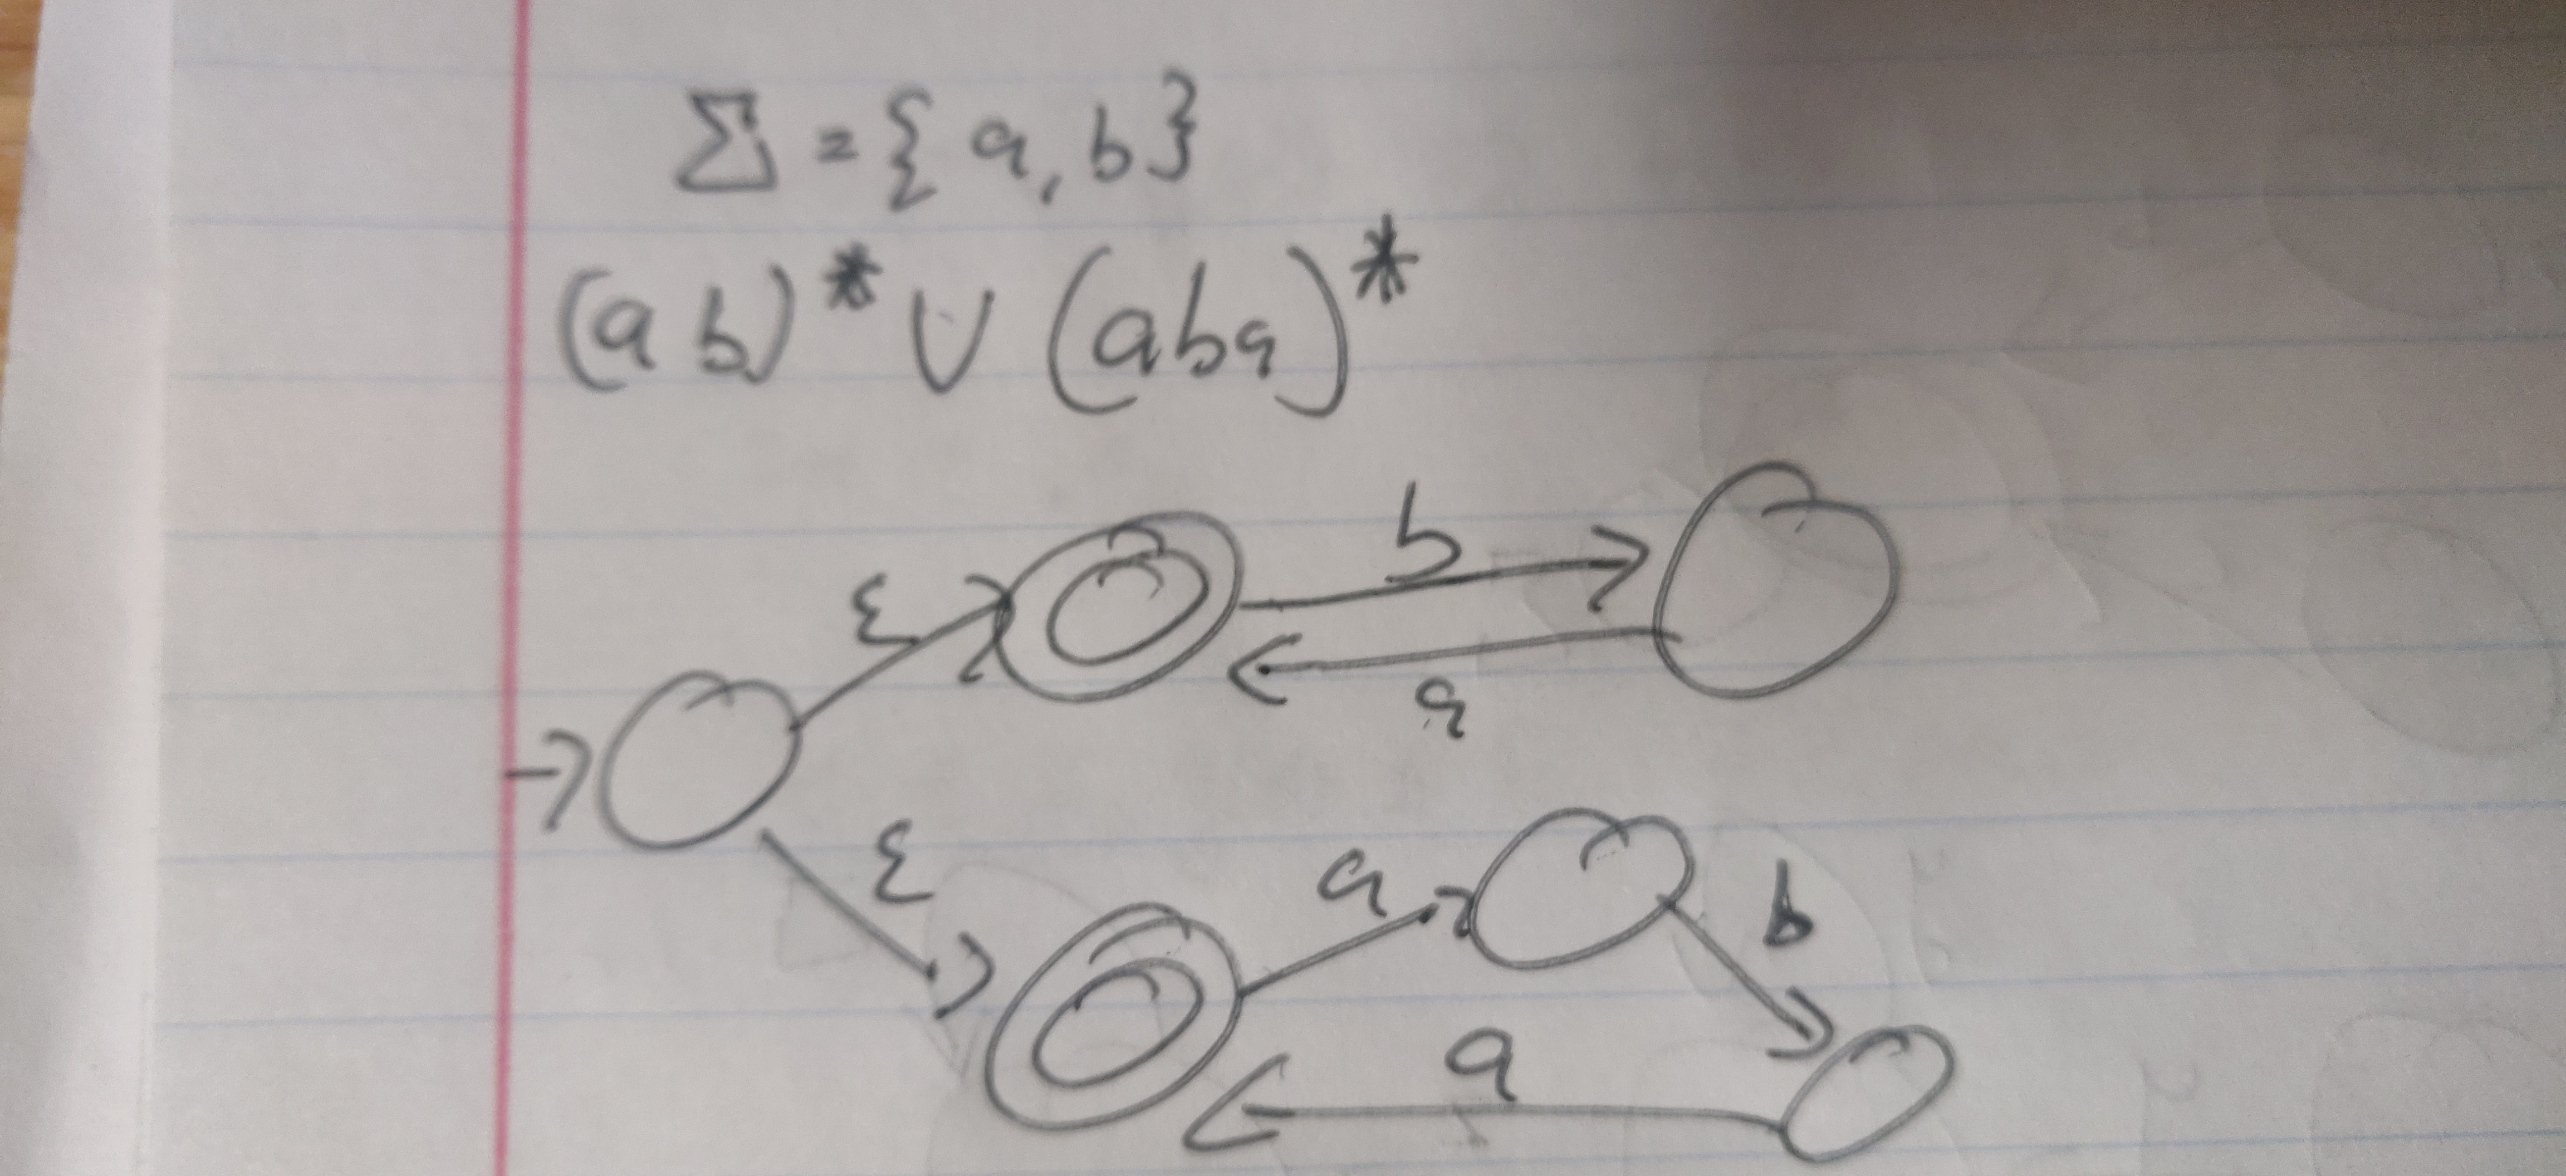
\includegraphics[width=5in]{3c.jpg}
    \end{align}
  \end{qparts}

  \newpage

  \q{55}{Working with an NFA}\\
  Consider the NFA $M = (Q, \Sigma, \delta, q_0, F)$ where:
  \begin{itemize}
    \item $Q = \{ 1, 2, 3, 4 \}$
    \item $\Sigma = \{ a, b \}$
    \item $\delta(q, s) =
            \begin{cases}
              \{2\}     & q = 1 \text{ and } s = a        \\
              \{1, 3\}  & q = 1 \text{ and } s = b        \\
              \{4\}     & q = 2 \text{ and } s = a        \\
              \{2, 3\}  & q = 4 \text{ and } s = \epsilon \\
              \emptyset & \text{otherwise}
            \end{cases}$
    \item $q_0 = 1$
    \item $F = \{ 2, 3 \}$
  \end{itemize}

  \begin{qparts}
    \item \emph{(20 pts)}
    Draw $M$ as a graph.
    \begin{solution}
    \end{solution}
    \begin{align}
      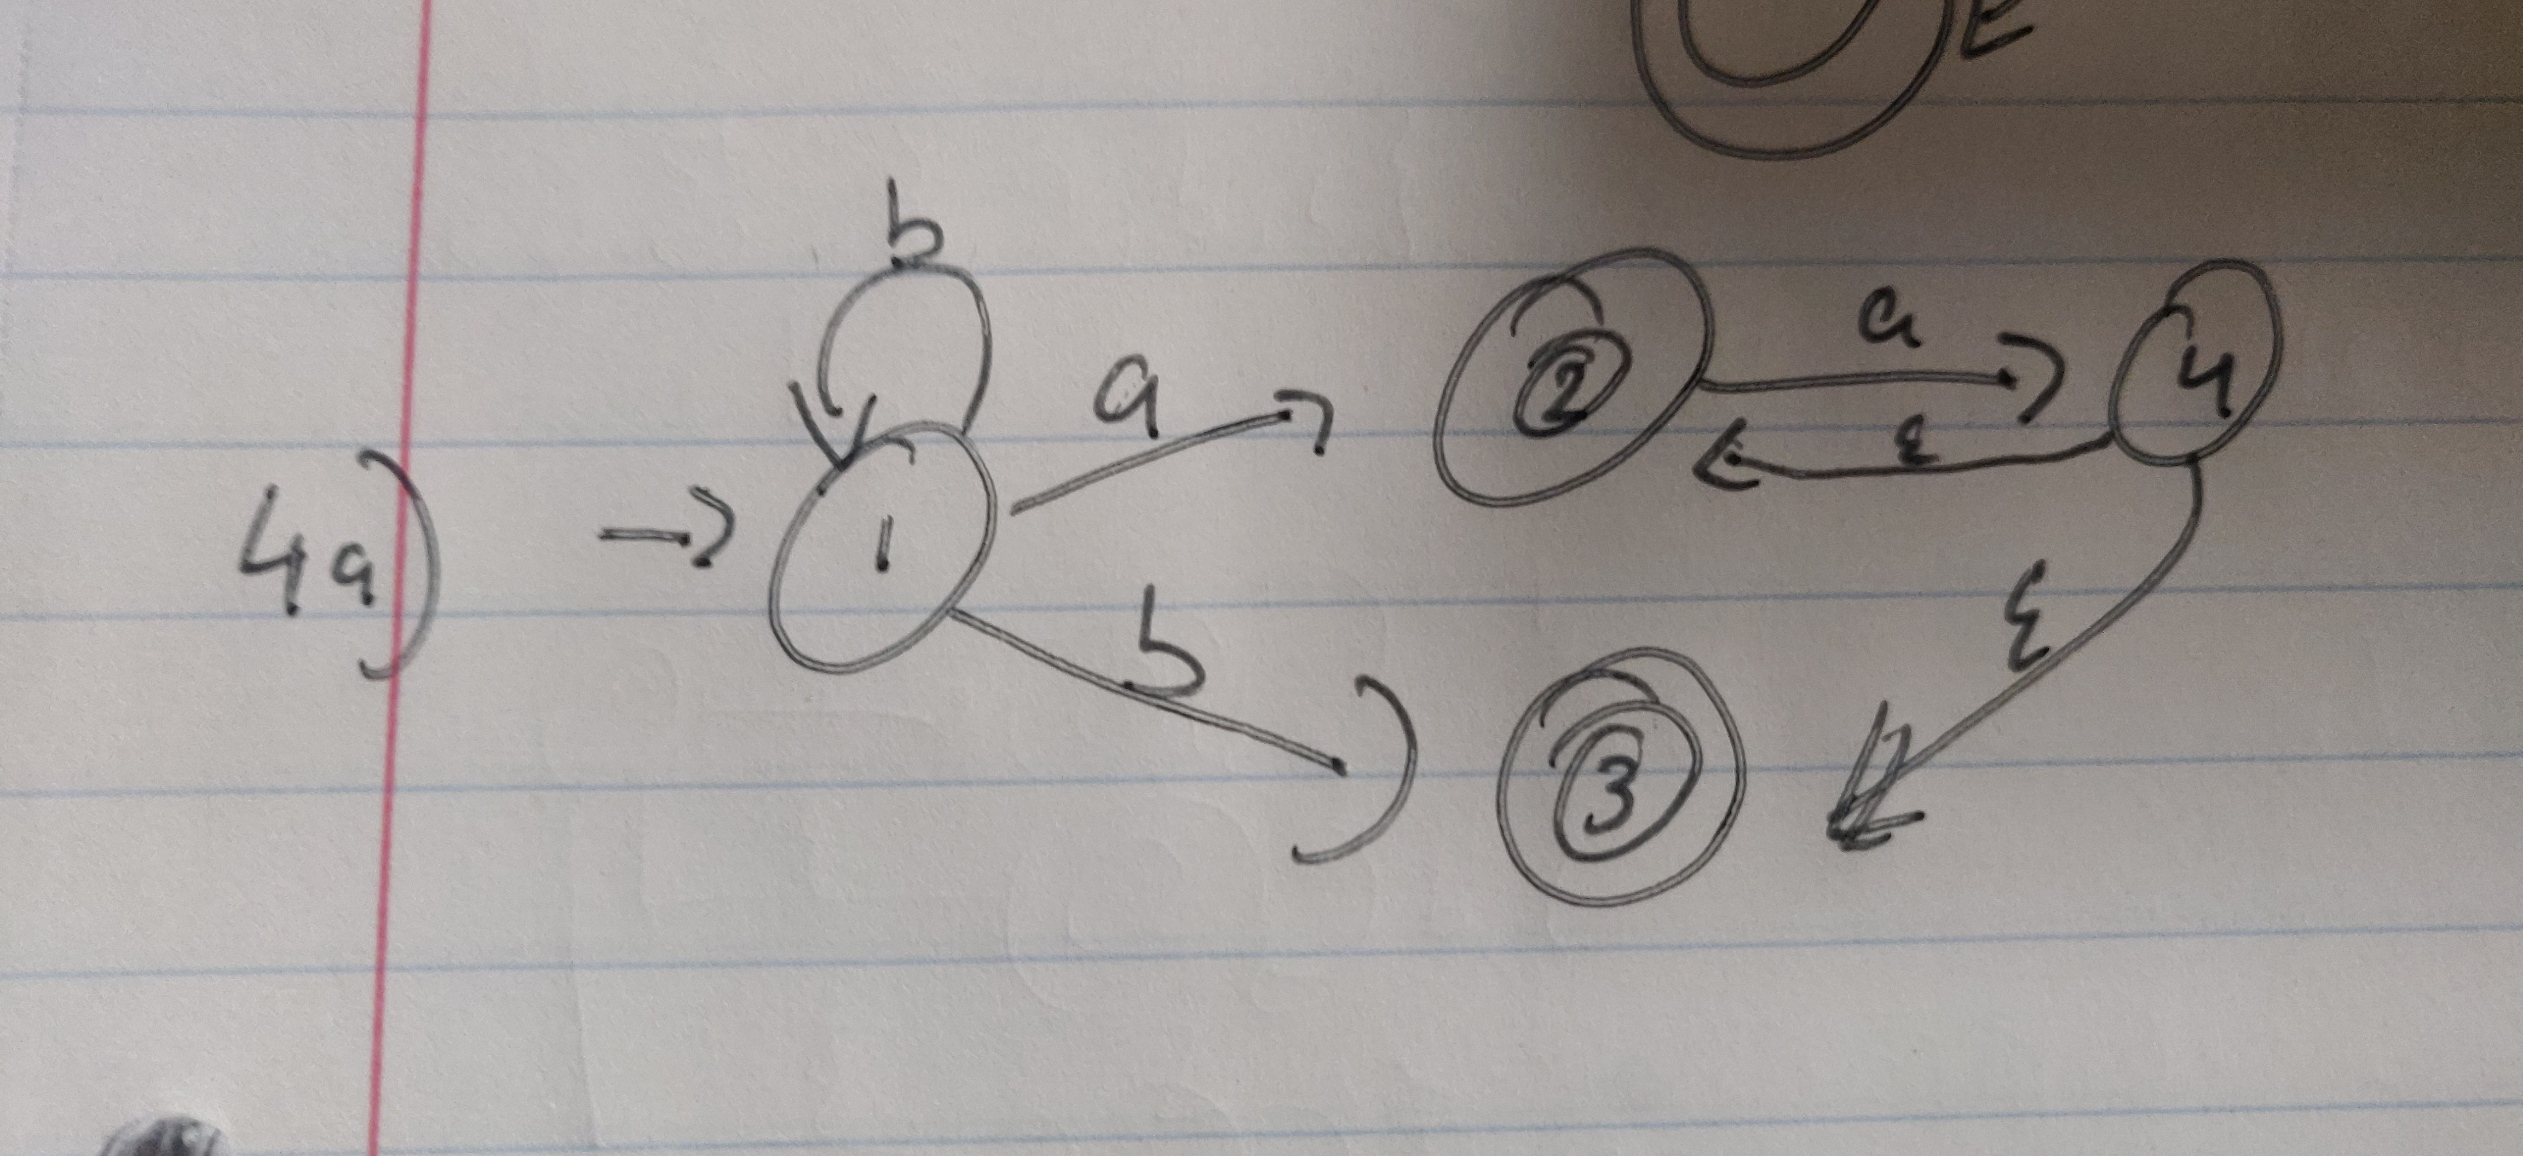
\includegraphics[width=5in]{4a.jpg}
    \end{align}
    \item \emph{(8 pts.)}
    What are the $\epsilon$-closures $E(\{1\})$, $E(\{2\})$, $E(\{4\})$, and $E(\{1, 4\})$?
    \begin{solution}
      \begin{gather}
        % \epsilon \Rightarrow Rejected\\
        E({1}) \Rightarrow {1}\\
        E({2}) \Rightarrow {2}\\
        E({4}) \Rightarrow {2,3,4}\\
        E({1,4}) \Rightarrow E({1}) \cup E({4}) = {1,2,3,4}
      \end{gather}
    \end{solution}
    \item \emph{(15 pts.)}
    Which of the following strings does $M$ accept: $\epsilon, aa, b, ba, aaabb$?
    Give an accepting path (just a sequence of states) for each accepted string.

    \begin{solution}
      \begin{gather}
        \epsilon \Rightarrow (1,\epsilon) \rightarrow ? \Rightarrow \mbox{  Rejected}\\
        aa \Rightarrow (1,a) \rightarrow (2,a) \rightarrow (4,\epsilon) \rightarrow 2 \Rightarrow \mbox{  Accepted}\\
        b \Rightarrow (1,b) \rightarrow 3 \Rightarrow \mbox{  Accepted}\\
        ba \Rightarrow (1,b) \rightarrow (1,a) \rightarrow 2 \Rightarrow \mbox{  Accepted}\\
        aaabb \Rightarrow (1,a) \rightarrow (2,a) \rightarrow (4,\epsilon) \rightarrow (2,a) \rightarrow (4,\epsilon) \rightarrow (2,b) \rightarrow ? \Rightarrow \mbox{  Rejected}
      \end{gather}
    \end{solution}

    \item \emph{(12 pts.)}
    What is the language $L(M)$ of $M$?
    \begin{solution}
      $L(M) = $ any string that has zero or more b's followed by zero or more a's.
    \end{solution}
  \end{qparts}

  \newpage

  \q{60}{Designing NFAs}\\
  For each of the following languages, draw an NFA (as a graph) recognizing it.
  Your NFAs should have no more than 4 states.
  \begin{qparts}
    \item
    All strings over $\Sigma = \{a, b, c, \dots, z\}$ containing either the substring $ab$ or the substring $bc$.
    \begin{solution}
    \end{solution}
    \begin{align}
      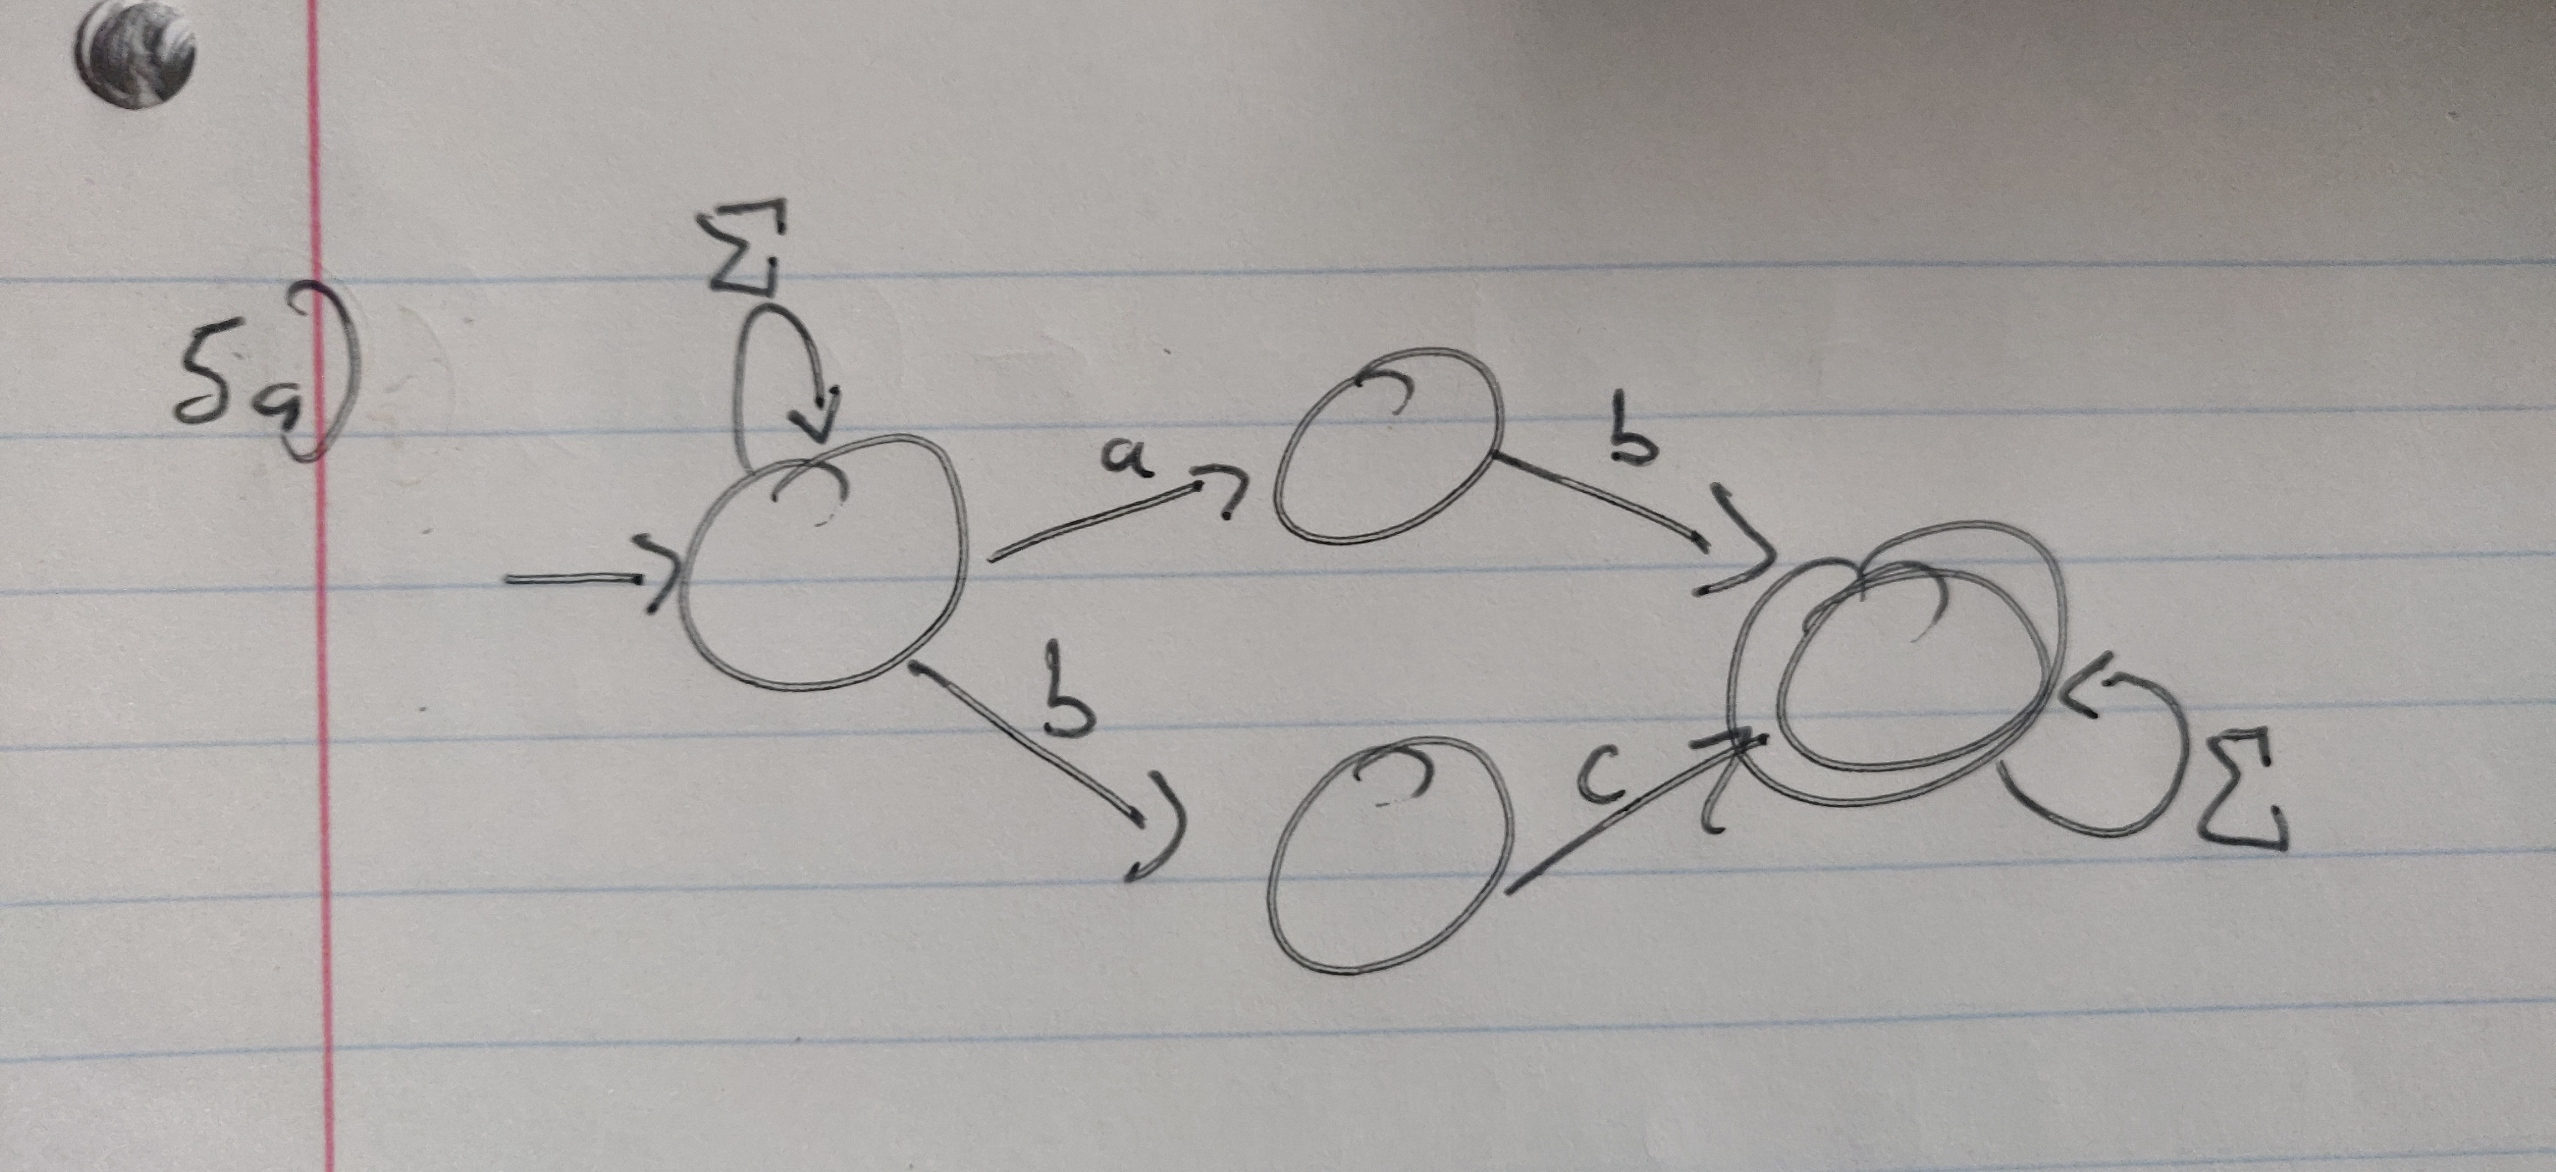
\includegraphics[width=5in]{5a.jpg}
    \end{align}
    \item
    All strings over $\Sigma = \{a, b, c, \dots, z\}$ which include a pair of $x$ and $z$ with only $y$s in between (e.g. $axyyzb$ and $xz$ are OK but $xaz$ and $xy$ are not).
    \begin{solution}
    \end{solution}
    \begin{align}
      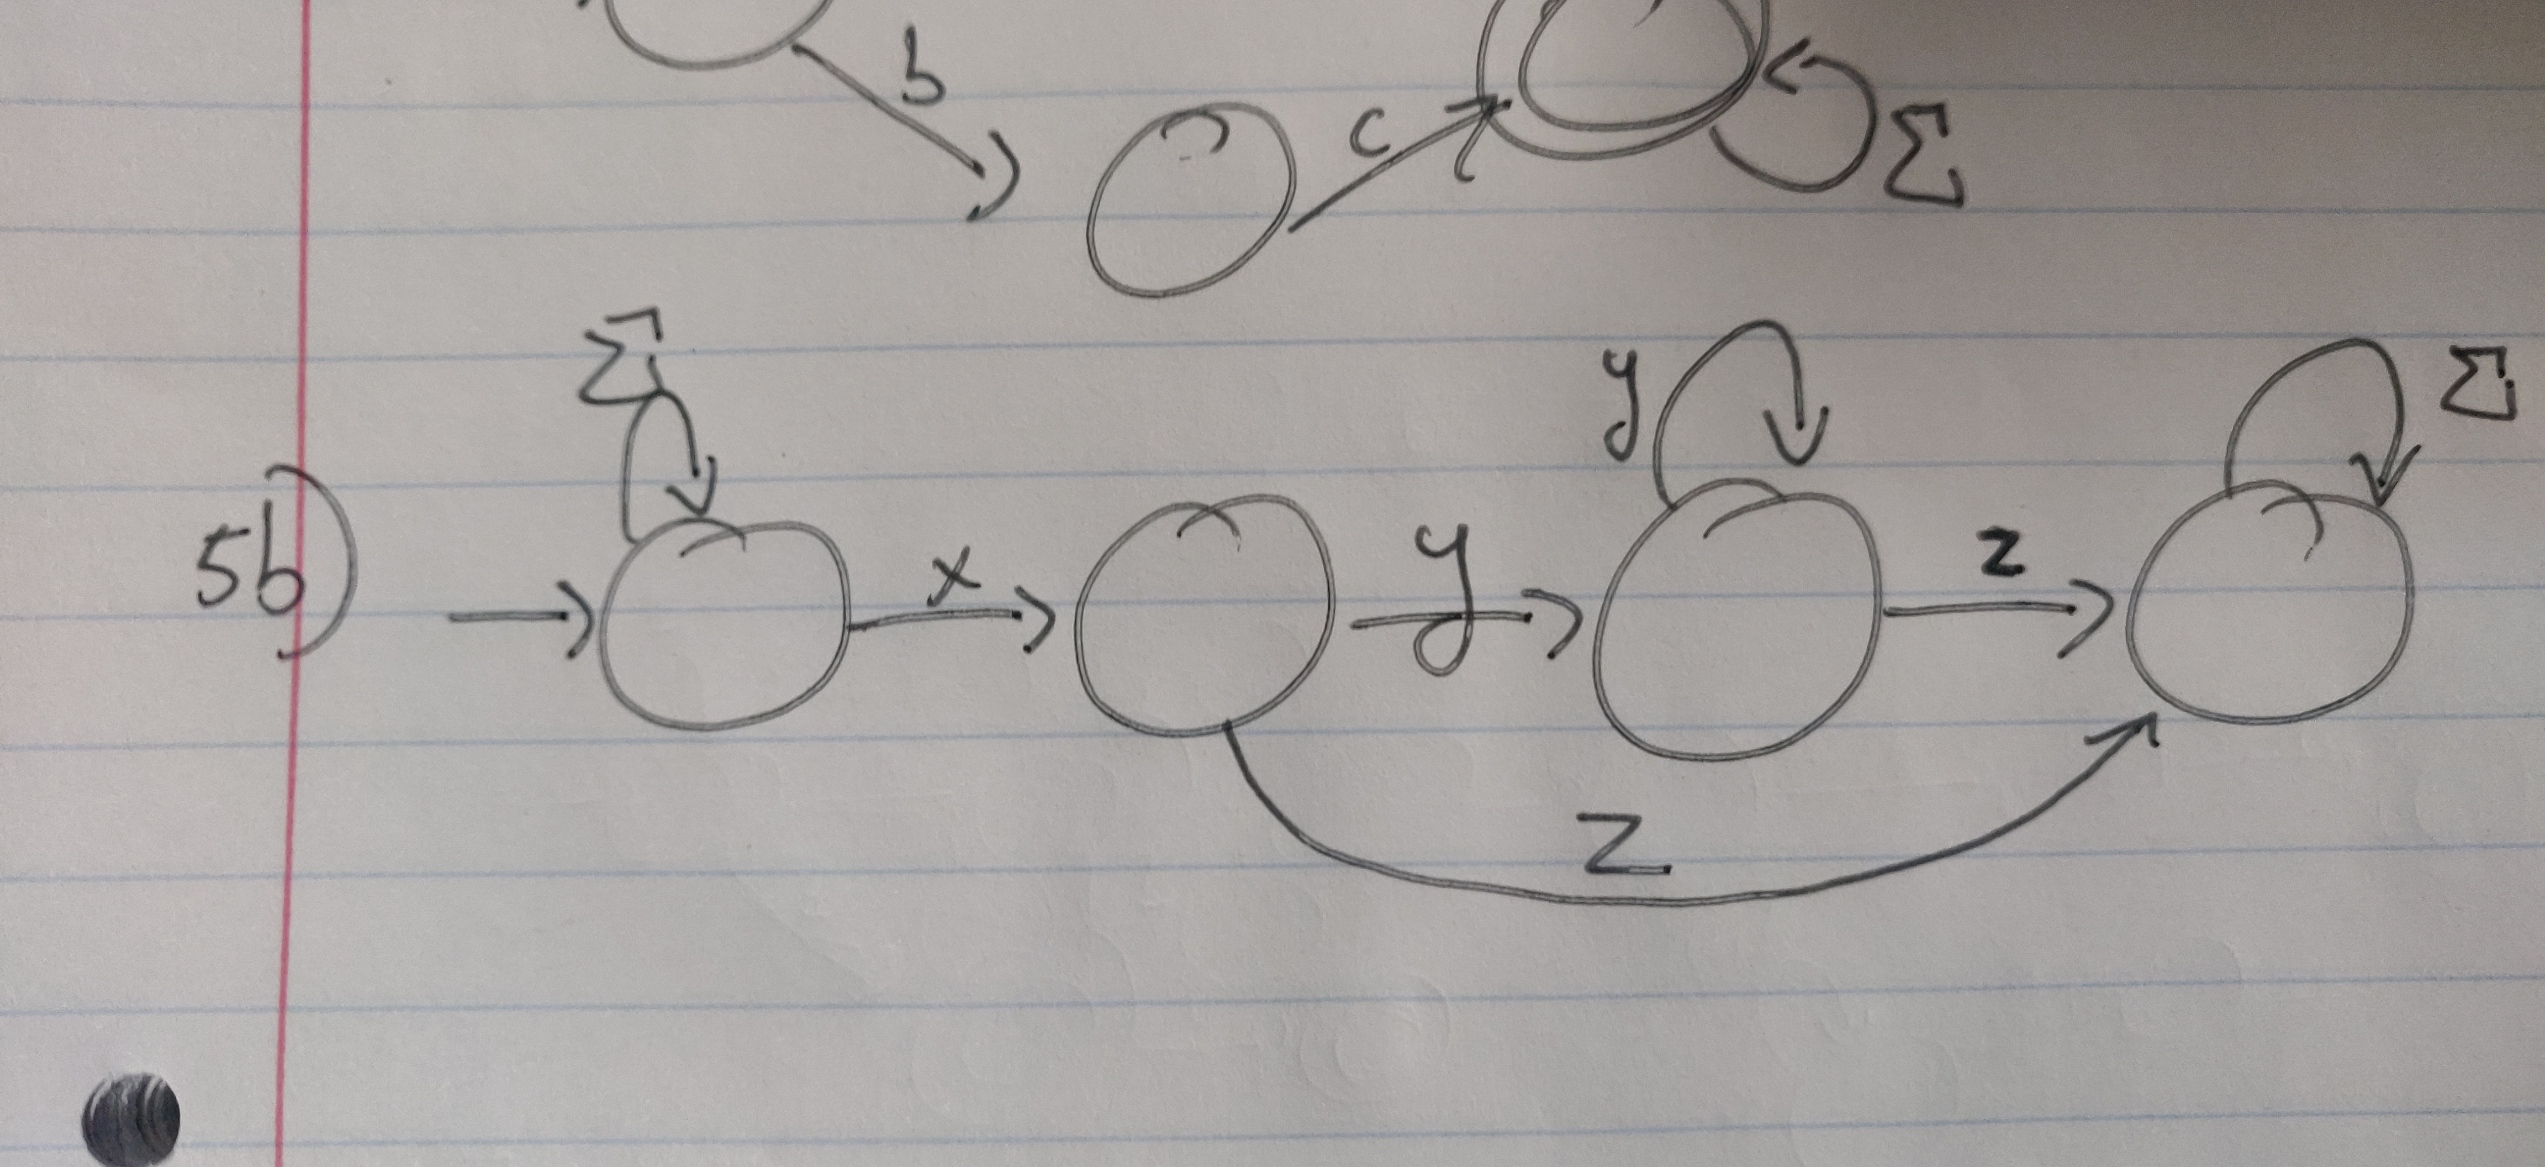
\includegraphics[width=5in]{5b.jpg}
    \end{align}
    \newpage
    \item
    All strings over $\Sigma = \{a, b, c\}$ which do not contain all three symbols (e.g. $aab$ and $bbba$ are OK but $bca$ is not).
  \end{qparts}
  \begin{solution}
  \end{solution}
  \begin{align}
    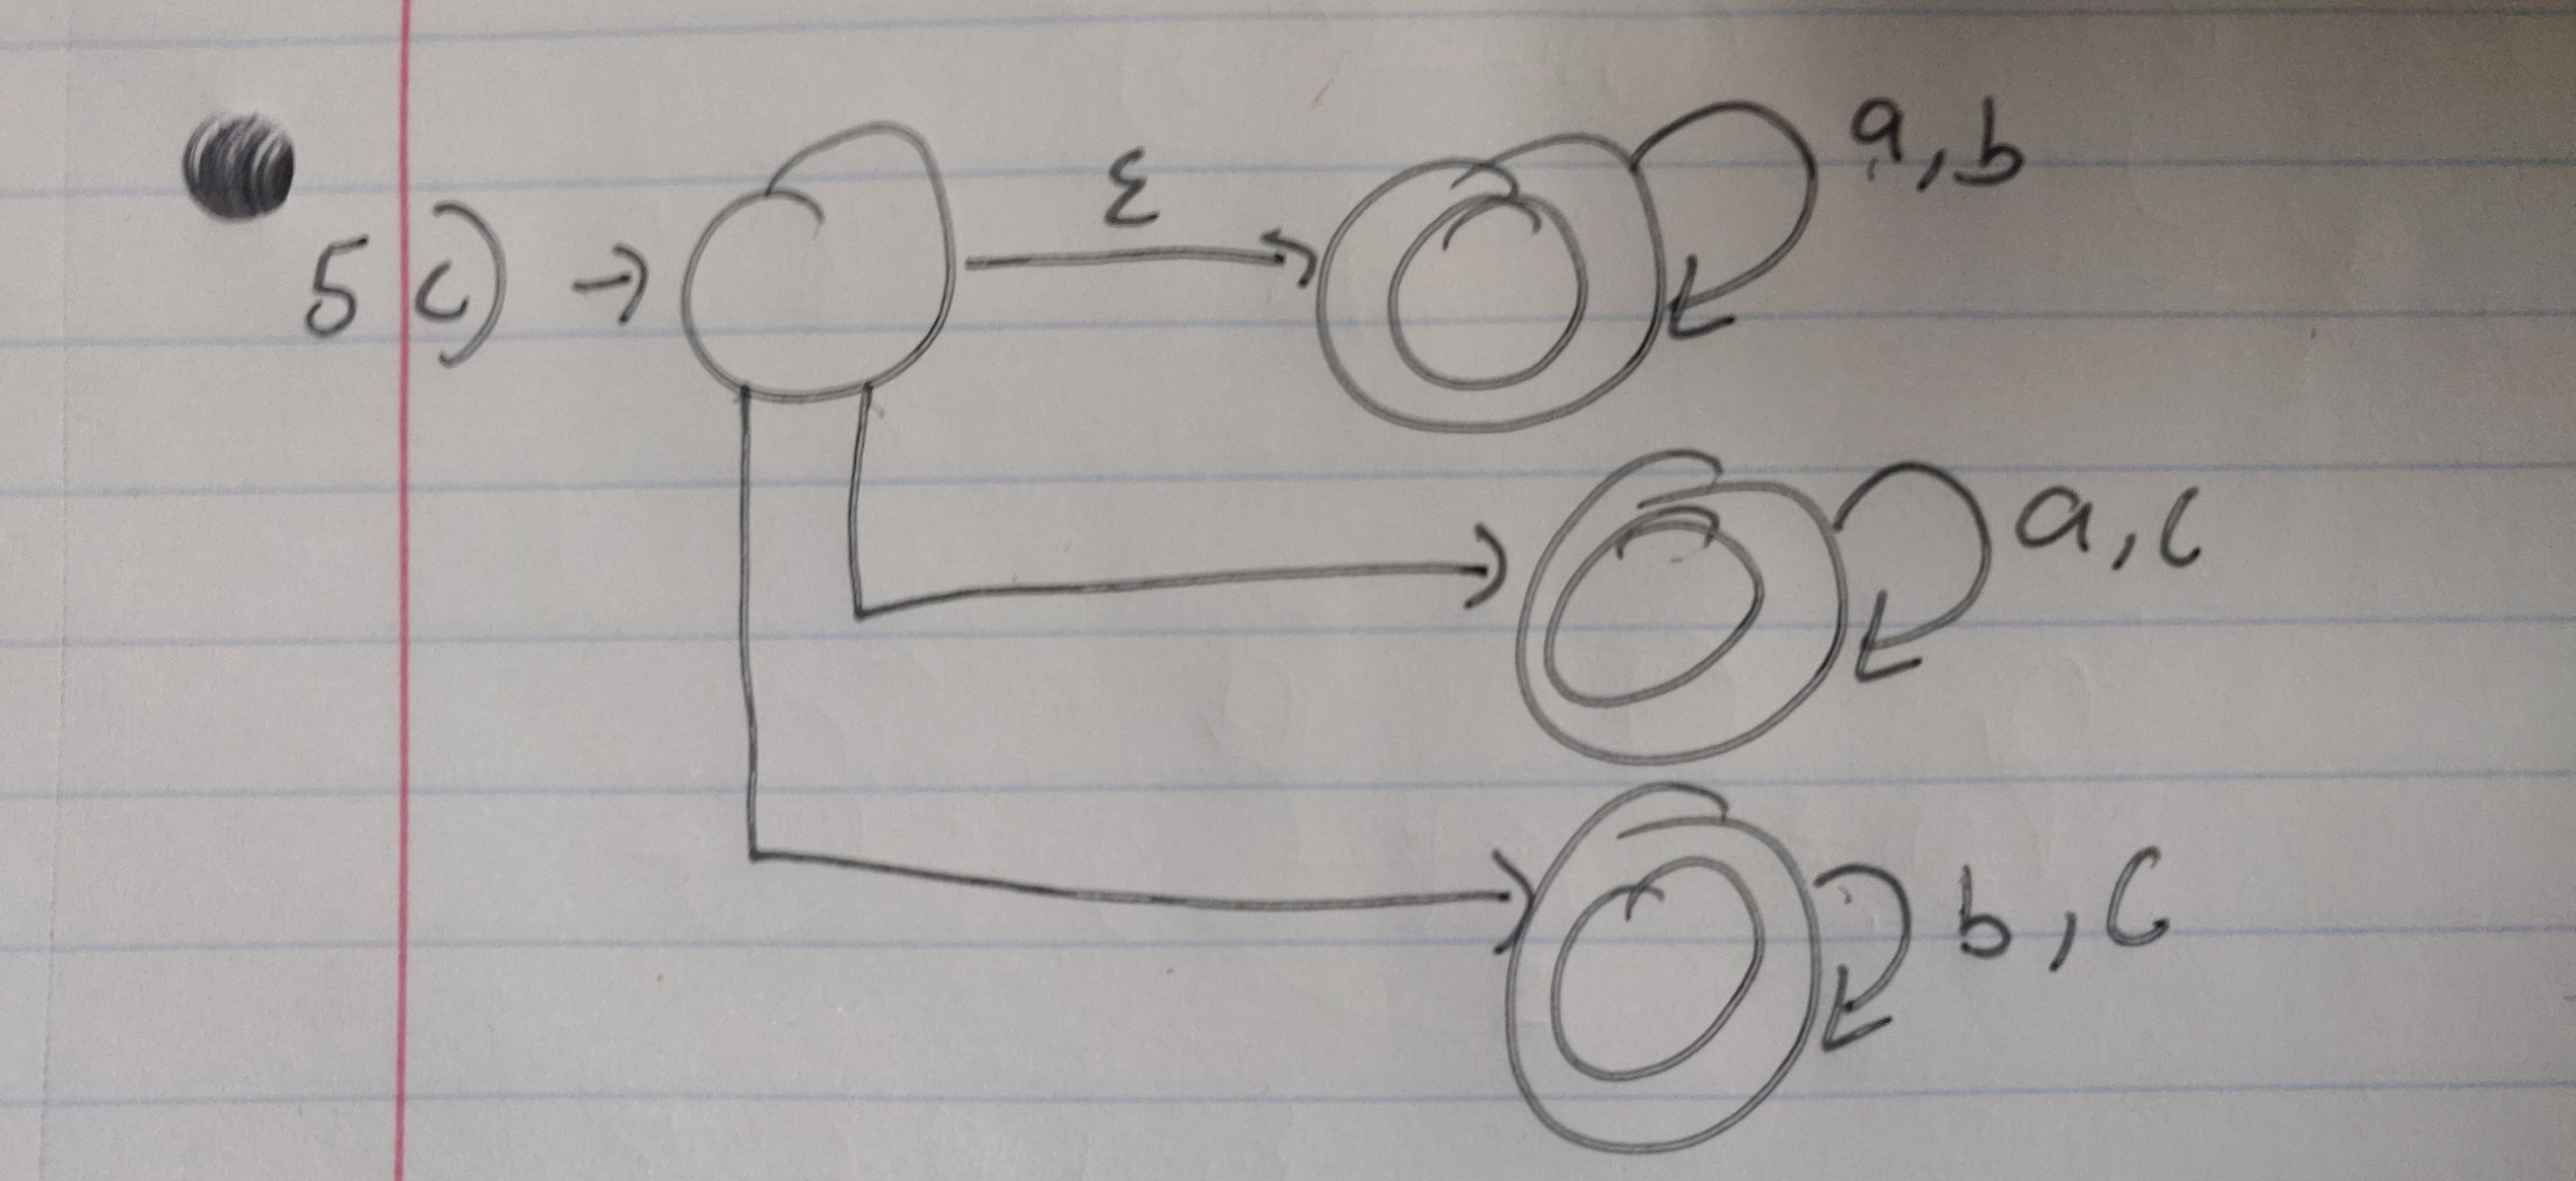
\includegraphics[width=5in]{5c.jpg}
  \end{align}
\end{qunlist}
\end{document}